\begin{comment}
Multicore architectures 
cache system
sharing and false sharing
existing tools for false sharing
limitations
contributions
structures
\end{comment}

Multicore processors are ubiquitous in the computing spectrum: from smart phones, personal desktops, to high-end servers. Multithreading is the de-facto programming model to exploit the massive parallelism of modern multicore architectures.
%Multithreading is widely used to employ these ubiquitous multicore processors for high parallelism. 
However, multithreaded programs may suffer from various performance issues caused by complex memory hierarchies~\cite{ibs-sc,ibs-sc2,Dramon}. Among them, false sharing is a common flaw that can significantly hurt the performance and scalability of multithreaded programs~\cite{falseshare:effect}. False sharing occurs when different threads, which are running on different cores with private caches, concurrently access logically independent words in the same cache line. When a thread modifies the data of a cache line, the cache coherence protocol (managed by hardware) automatically invalidates the duplicates of this cache line residing in the private caches of other cores~\cite{MESI}. Thus, even if other threads access completely different words inside this cache line, they have to reload the entire cache line from the shared cache or main memory. 

Unnecessary cache coherence caused by false sharing can dramatically degrade the performance of multithreaded programs, by up to an order of magnitude~\cite{falseshare:effect}. A concrete example shown in Figure~\ref{fig:penalty} also illustrates this catastrophic performance issue. We meant to employ multiple threads to accelerate the computation. However, when eight threads (on an eight-core machine) simultaneously access adjacent elements of {\tt array} sharing the same cache line, this program runs $\sim13\times$ slower (black bars) than its linear-speedup expectation (grey bars).
%The performance degradation caused by false sharing can be even more severe in modern architectures that integrate multiple sockets in chip; threads in different sockets involved in false sharing cause the cache coherence occurring in main memory not shared cache.
The hardware trend, such as adding more cores on chip and enlarging the cache line size, will further degrade the performance of multithreaded programs due to false sharing.
%, making the task of detection even more urgent. 

\begin{figure*}[htbp]
\centering
\subfigure[(a) A Program with False Sharing]{%
   \label{fig:penaltycode}
   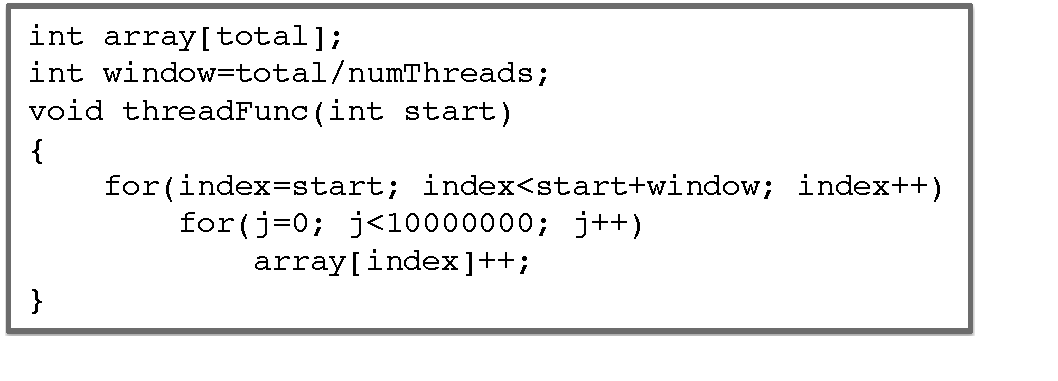
\includegraphics[width=3.1in]{figure/fscode}

}%
\hspace{20pt}
\subfigure[(b) Performance Degradation]{%
   \label{fig:penaltyfig}
   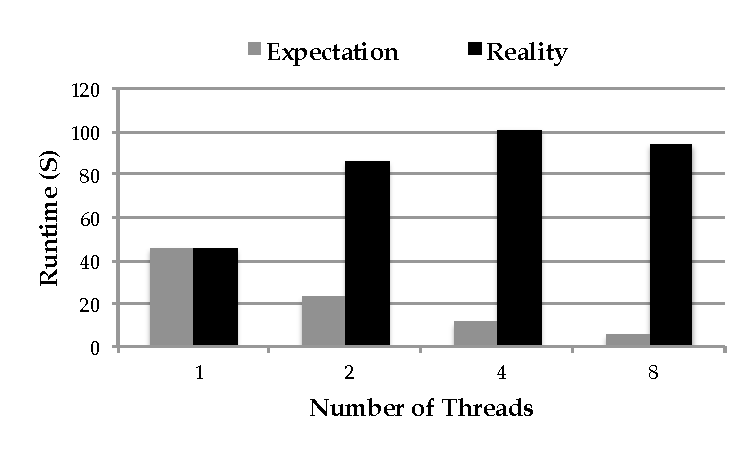
\includegraphics[width=3.1in]{figure/penalty}
}
\caption{
(a) A false sharing example inside a multithreaded program (b) causes $13\times$ performance degradation on an 8-core machine.
\label{fig:penalty}}
\end{figure*}

%\todo{Confirm the picture is readable in grey-style printing}

% Now we will talk about existing tools.
Unlike true sharing, false sharing is generally avoidable. When multiple threads unnecessarily share the same cache line, we can add byte paddings or utilize thread-private variables so that different threads can be forced to access different cache lines. Although the solution of fixing false sharing problems is somewhat straightforward, finding them is difficult and even impossible with manual checking, especially for a program with thousands or millions of lines of code. Thus, it is important to employ tools to pinpoint false sharing and provide insightful optimization guidance.

However, existing general-purpose tools do not provide enough details about false sharing~\cite{gprof, ibs-sc, Intel:VTune}. Existing false sharing detectors fall short in several ways. First, most tools cannot distinguish true and false sharing, or require substantial manual effort to identify optimization opportunities~\cite{falseshare:binaryinstrumentation1,detect:ptu,detect:intel,falseshare:binaryinstrumentation2,DProf, OSdetection, mldetect, Wicaksono11detectingfalse, openmp}. Second, tools~\cite{falseshare:binaryinstrumentation1,falseshare:binaryinstrumentation2,falseshare:simulator, Predator, qinzhao} based on memory access instrumentation introduce high runtime overhead, hindering their applicability to real, long-run applications. Third, some tools either require OS  extensions~\cite{OSdetection}, or only work on special applications~\cite{Sheriff}. Fourth, no prior tools assess the performance gain from eliminating an identified false sharing bottleneck. Without this information, many optimization efforts may yield trivial or no performance improvement~\cite{Sheriff, qinzhao}.

\Cheetah{} is designed to address all these issues with the following two contributions:
\begin{itemize} 

% The first one is overrated. We can't do that. 
\item {\bf The First Approach to Predict False Sharing Impact.} This paper introduces the first approach to predict the potential performance impact of fixing false sharing instances, without actual fixes. Based on our evaluation, \cheetah{} can precisely assess the performance improvement, with less than 10\% difference. By ruling out trivial instances, we can avoid unnecessary manual effort leading to little or no performance improvement. 

\item {\bf An Efficient and Effective False Sharing Detector.} \cheetah{} is an efficient false sharing detector, with only $\sim$7\% performance overhead. \Cheetah{} utilizes the performance monitoring units (PMUs) that are available in modern CPU architectures to sample memory accesses. \Cheetah{} provides sufficient information on false sharing problems, by pointing out the lines of code, names of variables, and detailed memory accesses involved in the false sharing. \Cheetah{} is a runtime library that is very convenient to be deployed; there is no need for a custom OS, nor recompilation and changing of programs. 

\end{itemize}

\begin{figure}[htbp]
\centering
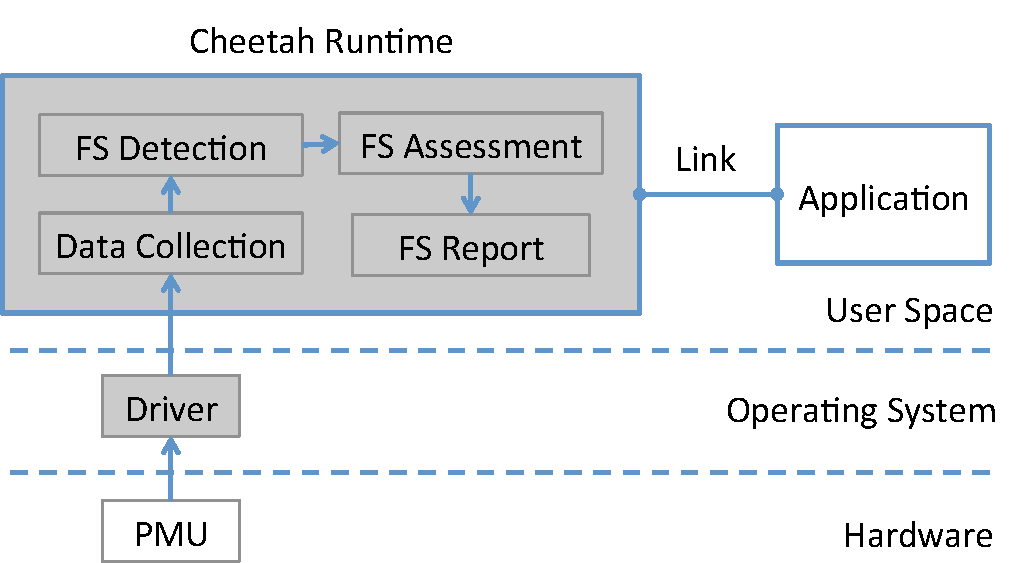
\includegraphics[width=1\columnwidth]{figure/cheetahcomponents}
\caption{Overview of \cheetah{}'s components (shadow blocks), where ``FS'' is the abbreviation for false sharing.}
\label{fig:components}
\end{figure}


%\cheetah{} is very convenient to use. There is no need to change or recompile programs, or to modify the underlying operating system. We evaluate \cheetah{} on two well-known benchmark suites, PARSEC~\cite{phoenix-hpca} and PHOENIX~\cite{parsec}. \cheetah{} successfully identifies significant false sharing problems, while skipping problems with only trivial or no performance improvement.

%
%is very convenient to use, which is a library that can be preloaded (using \texttt{LD\_PRELOAD} or can be linked to: there is no need to change or recompile the programs, or to modify the underlying operating system.
%\paragraph{\cheetah{} Overview}
Figure~\ref{fig:components} shows the overview of \Cheetah{}. 
%When the Performance Monitoring Unit (PMU) invokes an interrupt according to the pre-set sampling frequency, 
The ``data collection'' module gleans memory accesses via the address sampling supported by the hardware performance monitoring units (PMUs) and, with the assistance of the ``driver'' module, filters out memory accesses associated with heap or globals, feeding them into the ``FS detection'' module. At the end of an application, or when \cheetah{} is requested to report, the ``FS detection'' module examines the number of cache invalidations of each cache line, differentiates false sharing from true sharing, and passes false sharing instances to the ``FS assessment'' module. In the end, the ``FS report'' module only reports false sharing instances with a significant performance impact, along with its predicted performance improvement after fixes provided by the ``FS assessment'' module. 

%\Cheetah{} is has a co-design with hardware, operating system, and the user space programs. It monitors the memory accesses via the hardware performance monitoring unit (PMU) supported address sampling. By analyzing the address samples, \cheetah{} identifies significant false sharing problems (in FS-Detection component) and quantifies their impacts to the whole program execution (in FS-assessment component).
%'s components. When the Performance Monitoring Unit (PMU) invokes an interrupt according to the pre-set sampling frequency, the ``driver'' passes all information about a memory access to the ``data collection'' module residing in \Cheetah{}'s runtime system. Upon receiving this, the ``data collection'' module filters out memory accesses relating to heap or globals, and feeds them into the ``FS detection'' module. At the end of an application or when \cheetah{} is notified to report, ``FS detection'' will examine the number of cache invalidations of each cache line, differentiate false sharing from true sharing, and pass false sharing instances to the ``FS assessment'' module. Thus, ``FS report'' module only reports false sharing instances with significant performance impact, with its predicted performance improvement after fixes for every instance. 

%\paragraph{Paper Organization} 
The remainder of this paper is organized as follows. 
%Section~\ref{sec:overview} introduces the background of false sharing and the motivation of a new detection tool. 
Section~\ref{sec:detect} describes false sharing detection components of \Cheetah{}. Section~\ref{sec:predictimprove} discuesses how \cheetah{} assesses the performance impact of a false sharing instance. Section~\ref{sec:eval} presents experimental results, including effectiveness, performance overhead, and assessment precision. Section~\ref{sec:discuss} addresses main concerns about hardware dependence, performance, and effectiveness. Lastly, Section~\ref{sec:relatedwork} discusses related work, and Section~\ref{sec:conclusion} concludes this paper. 



